\section{Week 2}

\subsection{Lundi}

Lundi on a travaillé sur le logiciel CST. On a modelisé un antenne
dipolaire en or avec un substrat en Silicium sans pertes. L'idée
était un peu de jouer et de se familiariser avec le logiciel.

De ma part, j'ai varié le gap enter les deux brins pour obtenir le facteur S
en fonction de la fréquence pour plusieurs valeurs du gap. Cependant, j'ai oublié
de changer aussi la taille des brins. Cela veut dire qu'à chaque fois que je changeais
le gap, la taille totale de l'antenne changeait aussi. Or, il fallair changer le gap
en gardant la taille totale de l'antenne constante. J'ai pas eu le temps de corriger 
cette erreur.

\begin{wrapfigure}{R}{0.3\textwidth}
    \centering
    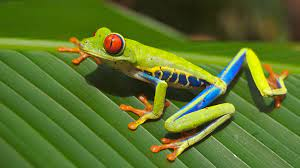
\includegraphics[width=0.25\textwidth]{texfigures/frog.jpg}
    \caption{\label{fig:frog1}This is a figure caption.}
\end{wrapfigure}

\subsection{Mardi}

Mardi on a travaillé sur le problème de l'enveloppe des signaux qu'on a obtenu la
seaine dernière. Victor a fait un code qui trouve les valeurs maximales en utilisant
\textsc{np.argmax}. Moi j'ai trouvé un code sur Stackexchange qui le fait en calculant
un changement de signe sur la dérivée du signal. 

Après il a commencé à travailler sur les antennes de papillon. Moi j'ai organisé tout et 
j'ai créé un github.